	\documentclass[aspectratio=43]{beamer}
\usepackage[english]{babel}
\input{chapters/preamble}

    \setbeamertemplate{background} 
    {
        \includegraphics[width=\paperwidth,height=\paperheight]{images/fond1.jpg}
    }
\title{Privacy Preserving Cryptographic Toolbox } %->->->->-> Check hyperref title <-<-<-<-<-
\subtitle{A survey with applications to Sovereign Identity}
\author[R. Dubois]{\textcolor{yellow}{Renaud Dubois}}
\institute[LIT]{
    \textcolor{white}{Ledger}%
    \\%
    \textcolor{white}{Innovation Team}%
} %You can change the Institution if you are from somewhere else
\date{\today}
%\logo{\includegraphics[width= 0.05\textwidth]{images/logo.png}}

\begin{document}
    
    \frame{\titlepage}
%%%%%%%%%%%%         
    \begin{frame}{Summary}
    
        \tableofcontents
        
%         Reed-Solomon Proximity (RP) Problem: Given oracle access to a Reed-Solomon code $f:S\rightarrow\mathbb{F}$, the Reed-Solomon Proximity Problem asks that a verifier $V$ distinguishes between two cases with high probability: \begin{itemize}
%                                                                                                                                                                                                                                           \item $$f\in \textbf{RS}[\mathbb{F},S,\rho]$$
%                                                                                                                                                                                                                                           \item $f$ is $\delta$-far pairwise Hamming distance from all $$f^\prime\in\textbf{RS}[\mathbb{F},S,\rho], f\neq f^\prime$$.
%                                                                                                                                                                                                                                          \end{itemize} 
   
    \end{frame} 
%%%%%%%%%%%% 
    \input{chapters/concepts.tex}
    
    %%%%%%%%%%%   
    \subsection{Anonymous Credentials}
  \begin{frame}{Anonymous Credentials}
  
  \begin{center}
  \includegraphics[width=8cm]{images/anonymouscredentials.jpg}
  \end{center}

  \end{frame}

 \begin{frame}{Anonymous Credentials Recipee}
 
 \begin{center}
 \textcolor{yellow}{\fbox{Ingredients}} 
 \end{center}

 \fbox{\parbox{\textwidth}{

 \begin{itemize} 
  \item Commitment : Digital sealed envelope, polynomial Commitment, Functional Commitment. Enables range-proof (Monero), serial number hiding (Zerocoin), universal proofs.
  \item Signatures with efficient protocols : Proof friendly, Structure Preserving, Group, Linkable \ldots
  \item Zero Knowledge Proof : proof a Knowledge of a value, without revealing it. From single value to universal.
 \end{itemize}
 }}
 
 \end{frame}
 
%%%%%%%%%%%%   
\input{chapters/toolbox.tex}
    

%%%%%%%%%%%%%%%%%%%%%%%%%%%%%%%%%%%%%%%%%%%%%     
 \begin{frame}{Pedersen Additive Homomorphic Commitment}
 totocs
 \end{frame}
 

\section{Pictures}
\begin{frame}
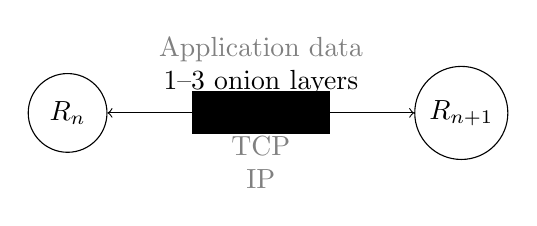
\begin{tikzpicture}

\node[circle,draw,minimum size=1cm] (R1) at (0, 0) {$R_n$};
\node[circle,draw,minimum size=1cm] (R2) at (5, 0) {$R_{n+1}$};

\draw[<->] (R1.east) -- node [midway, fill=black] (line) {\phantom{TLS layer}} (R2.west);

\node[align=center] at (line) {{\color{gray} Application data}\\1--3 onion
                    layers\\TLS layer\\{\color{gray}TCP}\\{\color{gray} IP}};

\end{tikzpicture}

\end{frame}
\begin{frame}



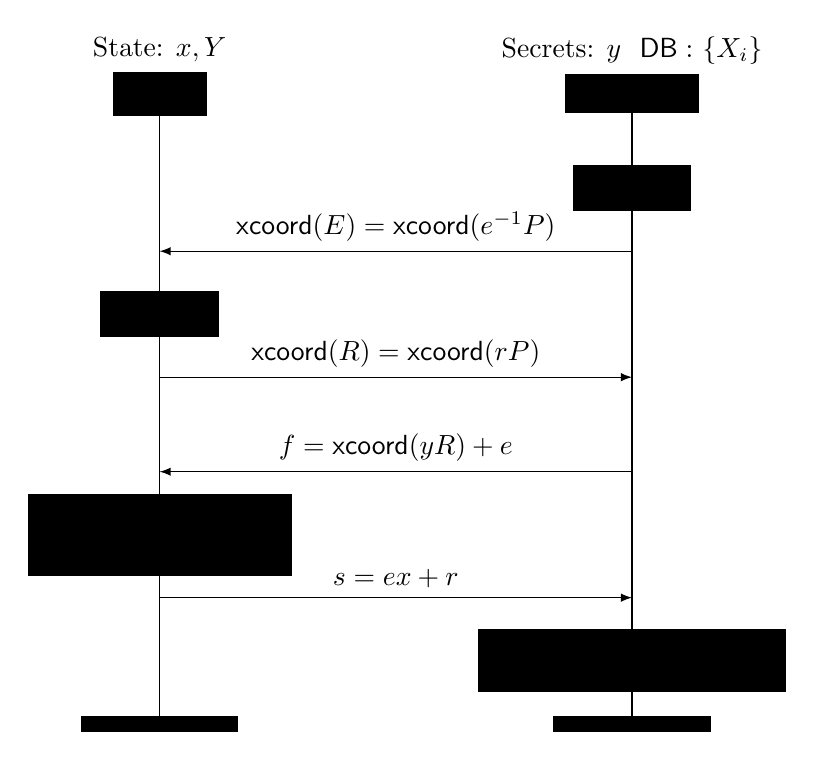
\begin{tikzpicture}[box/.style={draw,fill=black,align=center}]
\draw [line width=2mm] (0,0) -- ++(2,0) coordinate[midway](L1)
(6,0) -- ++(2,0) coordinate[midway](R1);
\draw (L1) -- ++ (0,8) 
node[box,pos=0.3] (L1a) {$e=f-\texttt{xcoord}(rY)$\\ $Ee\stackrel{?}{=}P$}
node[box,pos=0.65] (L1b) {$r\in_RZ_\ell^*$}
node[box,pos=1,label=above:{State: $x,Y$}] (L1c) {Tag $T$}
coordinate[pos=0.2] (X1) coordinate[pos=0.55] (X2);
\draw (R1) -- ++ (0,8) 
node[box,pos=0.1] (R1a) {$X=e^{-1}(sP-R)\stackrel{?}{\in}\mathsf{DB}$}
node[box,pos=0.85] (R1b) {$e\in_RZ_\ell^*$}
node[box,pos=1,label=above:{Secrets: $y$~~$\mathsf{DB}:$ $\{X_i\}$}] (R1c) {Reader $T$}
coordinate[pos=0.4] (X3) coordinate[pos=0.75] (X4);
\draw[-latex] (X1) -- (X1 -| R1) node[midway,above]{$s=ex+r$};
\draw[-latex] (X2) -- (X2 -| R1) node[midway,above]{$\mathsf{xcoord}(R)=\mathsf{xcoord}(rP)$};
\draw[-latex] (X3) -- (X3 -| L1) node[midway,above]{$f=\mathsf{xcoord}(yR)+e$};
\draw[-latex] (X4) -- (X4 -| L1) node[midway,above]{$\mathsf{xcoord}(E)=\mathsf{xcoord}(e^{-1}P)$};
\end{tikzpicture} 
 \end{frame}

 
%     \input{chapters/Blocksandcolors.tex}
%      
     \input{chapters/boxesandcolumns.tex}
    
    %\input{chapters/equationsandfigure.tex} 
    
    %\input{chapters/graphs.tex}
    
    
 %   \section*{References} %You can remove this if you do not want to use it
 %       \nocite{Djairo} \nocite{PhilPanof} \nocite{Fleming} \nocite{Shankar}
 %       \begin{frame}{References}
 %           \printbibliography
 %       \end{frame}

    \section{}
    \begin{frame}{}
        \centering
            \Huge\bfseries
        \textcolor{yellow}{Questions ?}
            \includegraphics[width=12cm]{images/questions.jpg}
     
    \end{frame}
\end{document}

% https://en.wikipedia.org/wiki/Privacy
% [CL16]: Concepts Around Privacy-Preserving Attribute-Based CredentialsJan Camenisch  https://hal.archives-ouvertes.fr/hal-01276046/document
